\documentclass[11pt,a4paper]{article}
\usepackage[utf8]{inputenc}
\usepackage{amsmath, amssymb, amsfonts}
\usepackage{algorithm}
\usepackage{algpseudocode}
\usepackage{graphicx}
\usepackage{booktabs}
\usepackage{kotex}
\usepackage{subcaption} % 여러 그림 배치를 위한 패키지
\usepackage{cite}


\title{양자 어닐링 기반 다중 밀집 사고 예방을 위한 보행자 네트워크 방향성 최적화}

\author{
    Quantum Guardian 팀\\
    컴퓨터공학부
}

\begin{document}

\maketitle

\begin{abstract}
군중 압착 사고는 좁은 도시 공간 내에서 서로 반대 방향으로 이동하는 조밀한 보행자 흐름이 한데 모일 때 발생하며, 이로 인해 개인의 이동성과 통제력이 상실될 수 있습니다. 본 연구는 보행자 네트워크를 위한 양자 어닐링(QA) 기반 방향성 최적화 프레임워크를 제안합니다. 보행자 네트워크는 가중치 그래프로 모델링되며, 최적화의 목적은 경로에 일방통행 방향을 할당하여 흐름 충돌을 줄이고 이동 효율성을 높이는 것입니다. 이를 위해 (i) 전역 연결성 유지를 위한 전처리, (ii) 이동 거리 단축을 위한 n-hop 기반 근사, (iii) 노드별 유량 보존 전략을 통합한 QUBO 모델을 정형화하였습니다. 실험 결과, 제안된 방법은 시뮬레이션 어닐링 대비 향상된 유량 안정성과 낮은 APSP 합계를 기록하였으며, 실제 양자 어닐러를 통한 검증 계획을 포함하고 있습니다.
\end{abstract}

\section{서론}
이태원 참사와 같은 압사 사고는 좁은 공간 내에서 보행자 흐름의 '군중 유체화 현상'으로 인해 발생합니다. 특히 대향류(Opposing flows)의 충돌은 개인의 이동성을 상실시키고 정체를 유발하게 됩니다. 본 연구는 양방향 보행로를 최적의 단방향 네트워크로 전환하여 흐름의 충돌을 방지하고 전체 네트워크의 이동 효율성을 극대화하는 것을 목적으로 합니다.

\section{수학적 문제 정의}

\subsection{그래프 표현 및 결정 변수}
보행자 네트워크를 무방향 그래프 $G = (V, E)$로 정의합니다. 각 간선의 방향을 결정하기 위해 $i < j$인 모든 간선 $(i, j) \in E$에 대해 이진 변수 $x_{ij} \in \{0, 1\}$를 정의합니다. $x_{ij}=0$은 $i \to j$, $x_{ij}=1$은 $j \to i$ 방향을 의미합니다. 특정 방향 흐름 $i \to j$의 존재 여부를 나타내는 지표 함수 $I_{i \to j}$는 다음과 같습니다:
\begin{equation}
    I_{i \to j} = 
    \begin{cases} 
    1 - x_{ij}, & i < j \text{ 인 경우} \\
    x_{ji}, & i > j \text{ 인 경우}
    \end{cases}
\end{equation}

\section{연결성 유지를 위한 전처리 (Preprocessing)}
    \subsection{면 분할(Face Partitioning)의 도입 배경}
    도로망 그래프의 전역적 연결성(Global Connectivity)을 보장함과 동시에 양자 최적화 모델의 실효성을 확보하기 위해, 해당 전처리 과정에서는 대상 도로망을 여러 개의 거대 면(Macro-Face)으로 묶어 최적화하는 면 분할 기법을 도입합니다.
    
    \subsubsection{분할 정복}
    현재의 양자 하드웨어는 사용할 수 있는 큐비트(Qubit)의 개수에 제한이 있습니다. 따라서 도로망의 모든 간선을 개별 변수로 삼아 단일 QUBO 모델을 구성할 경우, 그래프의 규모가 커짐에 따라 필요한 큐비트 수가 하드웨어의 수용 한계를 쉽게 초과하게 됩니다. 
    
    이러한 물리적 제약 하에서도 연산을 가능하게 만들기 위해, 전처리 단계에서는 분할 정복(Divide and Conquer) 전략을 활용합니다. 인접한 단위 면들을 묶어 여러 개의 거대 면(Sub-graph)으로 군집화하고, 최적화 변수를 전체 간선이 아닌 각 Sub-graph의 내부 간선들로 분할하여 개별적으로 최적화를 수행합니다. 이를 통해 한 번의 연산에 요구되는 큐비트의 수를 가용 범위 내로 축소하여 최적화 모델의 실행 가능성을 확보합니다.
    
    \subsection{거대 면 분할 알고리즘의 수행 절차}
    거대 면 분할은 평면 그래프의 기하학적·위상적 특성을 바탕으로 다음과 같은 알고리즘을 거쳐 수행됩니다. 이때, 사용자가 지정하는 하이퍼파라미터 $k$(목표 분할 개수)를 통해 문제의 규모와 하드웨어 환경에 맞는 유연한 분할이 가능합니다.
    
    \subsubsection{기하학적 면 구조 기반의 공간 클러스터링}
    도로망을 평면 그래프로 모델링한 뒤, 내부의 모든 단위 면을 추출하고 각각의 중심 좌표를 계산합니다. 이후 지정된 목표 분할 수 $k$개만큼 서로 거리가 먼 시드 면들을 초기 설정합니다. 이 시드들을 중심으로, 쌍대 그래프를 활용하여 주변 면들을 점진적으로 병합해 나가는 확장 알고리즘을 실행하여 전체 그래프를 $k$개의 군집으로 분할합니다.
    
    \subsubsection{외곽선 보정 (Wall-Protected Repair)}
    단순 확장 과정에서 각 군집의 경계선이 닫히지 않거나, 그래프 바깥쪽 외곽으로 영역이 누출되는 현상이 발생할 수 있습니다. 이를 방지하기 위해 외벽 간선에 극도로 높은 페널티 가중치를 부여한 상태에서 최소 비용 수리(T-join Repair)를 진행합니다. 내륙 간선만을 이용해 끊어진 경계를 최적의 경로로 이어붙임으로써, 독립된 $k$개의 닫힌 거대 면 구조를 최종 완성합니다.
    
    \subsection{시간 복잡도(Time Complexity) 분석}
    해당 전처리 과정은 방대한 탐색 공간을 줄이기 위한 것으로, 다항 시간 내에 신속하게 수행됩니다. 정점의 수를 $|V|$, 간선의 수를 $|E|$, 최소 단위 면의 수를 $|F|$라 하고, 경계선 보정 과정에서 탐색이 필요한 홀수 차수 정점의 수를 $|K_{odd}|$라 할 때 연산 소요 시간은 다음과 같습니다.
    
    \begin{itemize}
        \item 평면 임베딩 및 면 추출: $O(|V|)$
        \item 쌍대 그래프 생성 및 확장 알고리즘 병합: $O(|F|)$
        \item 경계선 보정을 위한 최단 경로 탐색 및 Blossom 매칭 연산: $O(|K_{odd}| \cdot |E| \log |V| + |K_{odd}|^3)$
    \end{itemize}
    
    이를 종합한 전체 시간 복잡도는 $O(|V| + |K_{odd}| \cdot |E| \log |V| + |K_{odd}|^3)$으로 도출됩니다. 실제 분할 과정에서 발생하는 경계선 상의 홀수 정점 수 $|K_{odd}|$는 전체 정점 수에 비해 매우 작기 때문에, 대규모 그래프에서도 지연 없이 빠른 처리가 가능합니다.
    
    \subsection{실효성 검증}
    
    \begin{figure}[htbp!]
        \centering
        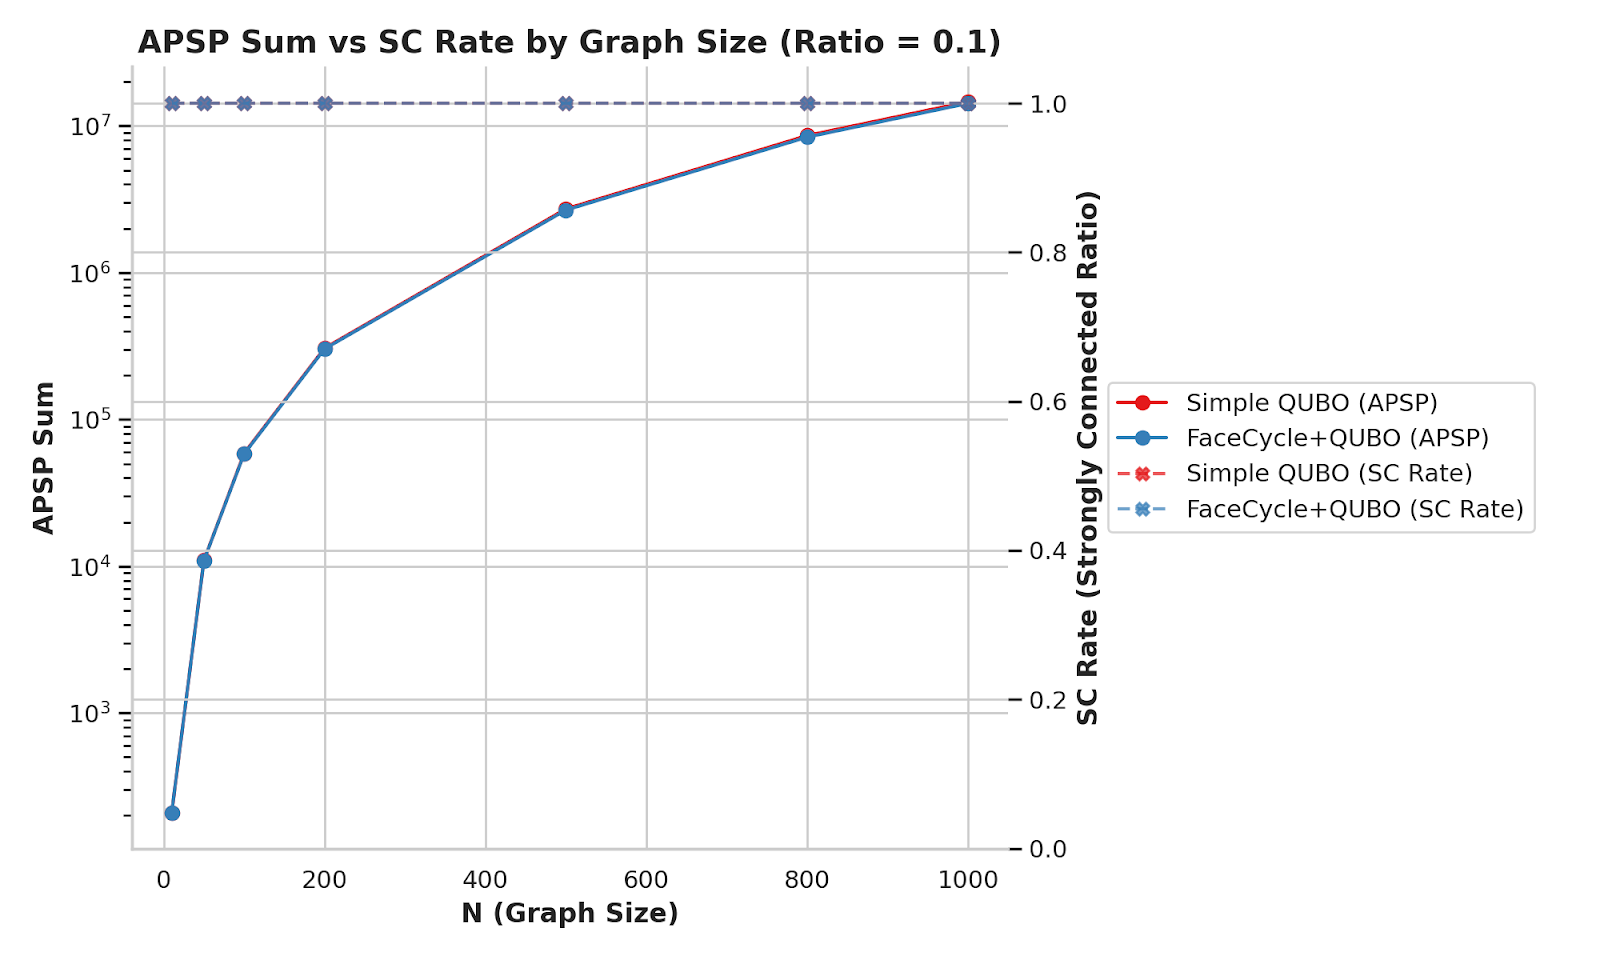
\includegraphics[width=0.8\textwidth]{remove_ratio_10.png} \\ \vspace{0.5cm}
        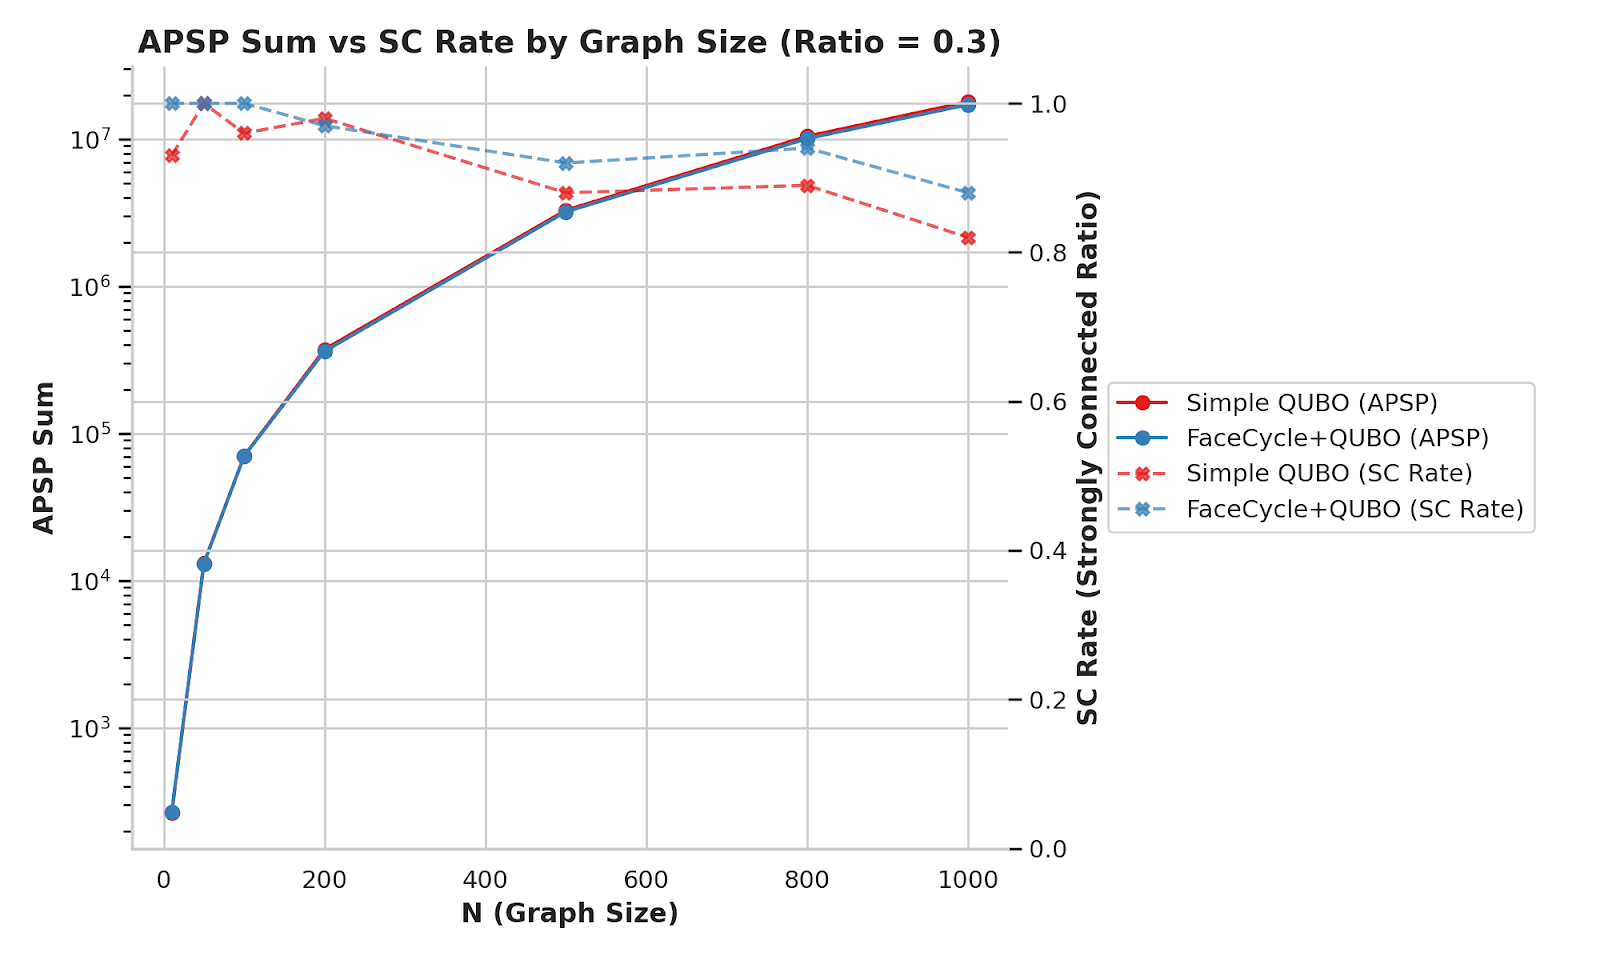
\includegraphics[width=0.8\textwidth]{remove_ratio_30.png} \\ \vspace{0.5cm}
        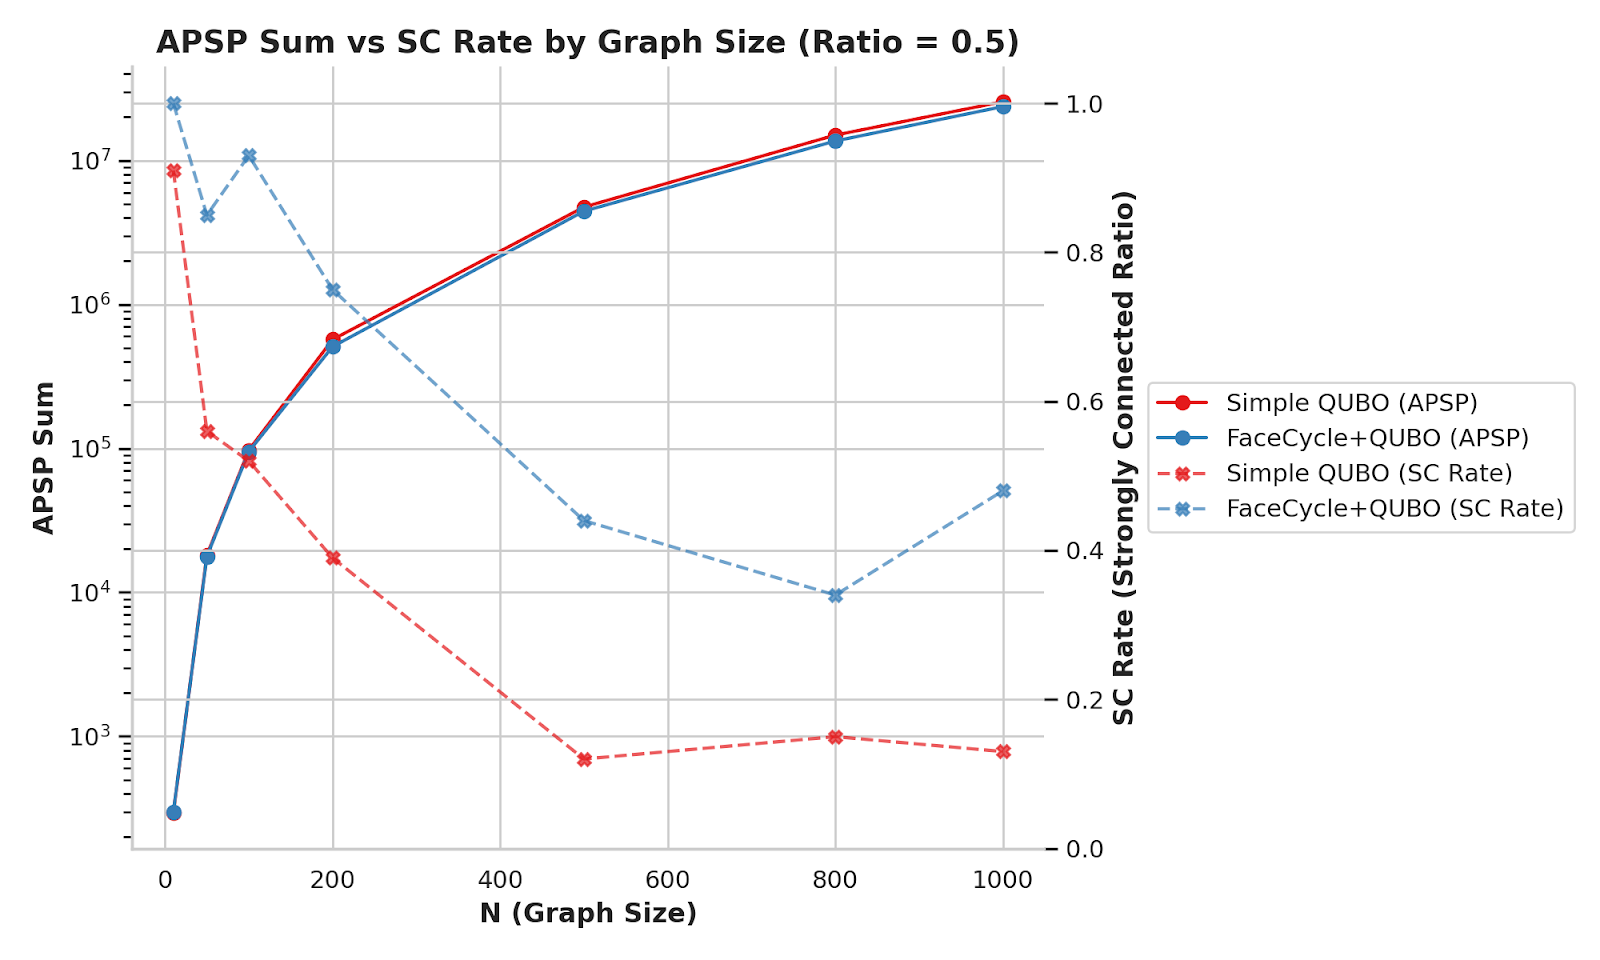
\includegraphics[width=0.8\textwidth]{remove_ratio_50.png}
        \caption{무작위 간선 삭제 비율(remove\_ratio)에 따른 APSP Sum 및 SC Rate 변화}
        \label{fig:remove_ratio_results}
    \end{figure}
    
    본 알고리즘의 실효성 검증을 위해 들로네 삼각분할(Delaunay Triangulation) 그래프에서 무작위 간선 삭제 비율에 따른 최단 경로 거리 합(APSP Sum)과 강결합 컴포넌트 비율(SC Rate)을 측정했습니다.
    
    실험 결과, 간선 삭제 비율이 낮은 환경(remove\_ratio = 0.1)에서는 두 방식 간의 성능 차이가 거의 없었으나, 그래프의 희소성이 증가하는 환경(remove\_ratio = 0.3, 0.5)에서는 전처리 기법의 강점이 명확히 드러납니다. 단순 QUBO 방식은 그래프 규모가 커질수록 SC Rate가 0.2 이하로 급락하여 전역적 연결성을 상실하는 반면, 전처리 모델은 상대적으로 높은 연결 비율을 방어하면서도 단순 방식과 유사한 최단 경로 효율(APSP Sum)을 유지합니다.
    
    결론적으로 이는 제안하는 전처리 기법이 간선이 부족하고 제약이 많은 열악한 도로망 환경에서 필수적인 전역적 연결성을 안정적으로 보장함을 입증합니다.
    
\section{QUBO 목적 함수 설계}
최소화할 총 에너지 함수 $H_{total}$은 유량 보존($H_{flow}$)과 이동 효율성($H_{dist}$)의 합으로 구성됩니다:
\begin{equation}
H_{total} = \alpha H_{flow} + \beta H_{dist}
\end{equation}

\subsection{유량 보존 항 ($H_{flow}$)}
각 정점 $v$에서의 유입량과 유출량 균형을 맞추기 위해 다음 페널티 항을 부과합니다:
\begin{equation}
H_{flow} = \sum_{v \in V} \left( \sum_{u \in adj(v)} (2 \cdot I_{v \to u} - 1) \right)^2
\end{equation}

\subsection{이동 효율 최적화 항 ($H_{dist}$)}
APSP(All-Pairs Shortest Paths)를 직접 최적화하는 것은 높은 차수의 다항식을 유발하므로, 본 연구에서는 $n$-hop 경로 수의 최대화를 대리 지표로 활용합니다.

\begin{figure}[t]
    \centering
    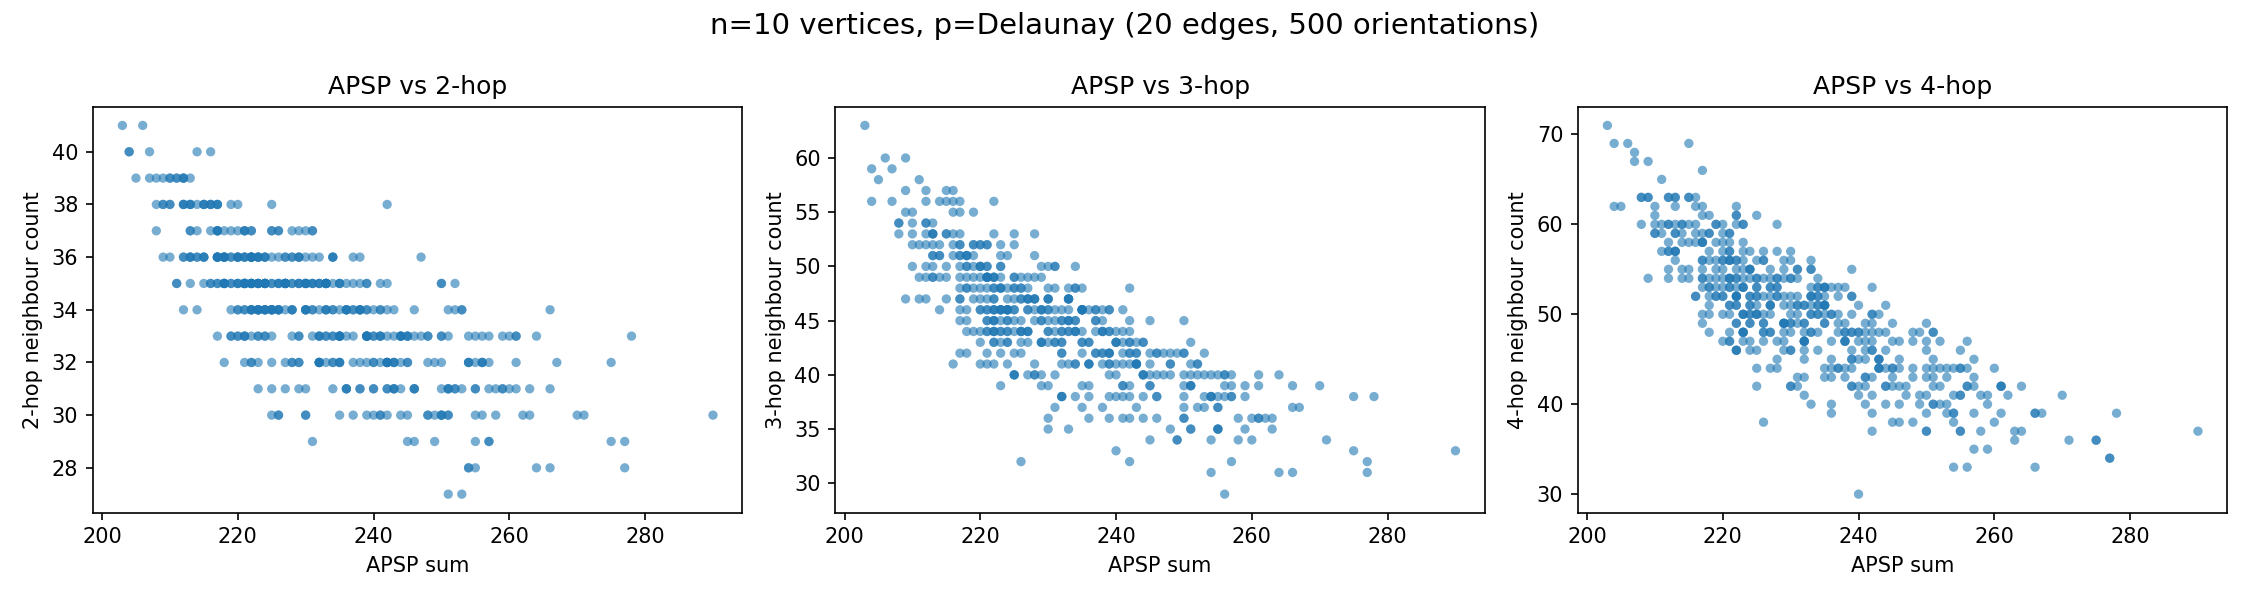
\includegraphics[width=0.85\textwidth]{result_v10_Delaunay.png}
    \caption{$n=10$에서의 n-hop 이웃 수 합과 APSP 총합의 상관관계}
    \label{fig:n10}
\end{figure}    

\begin{figure}[t]
    \centering
    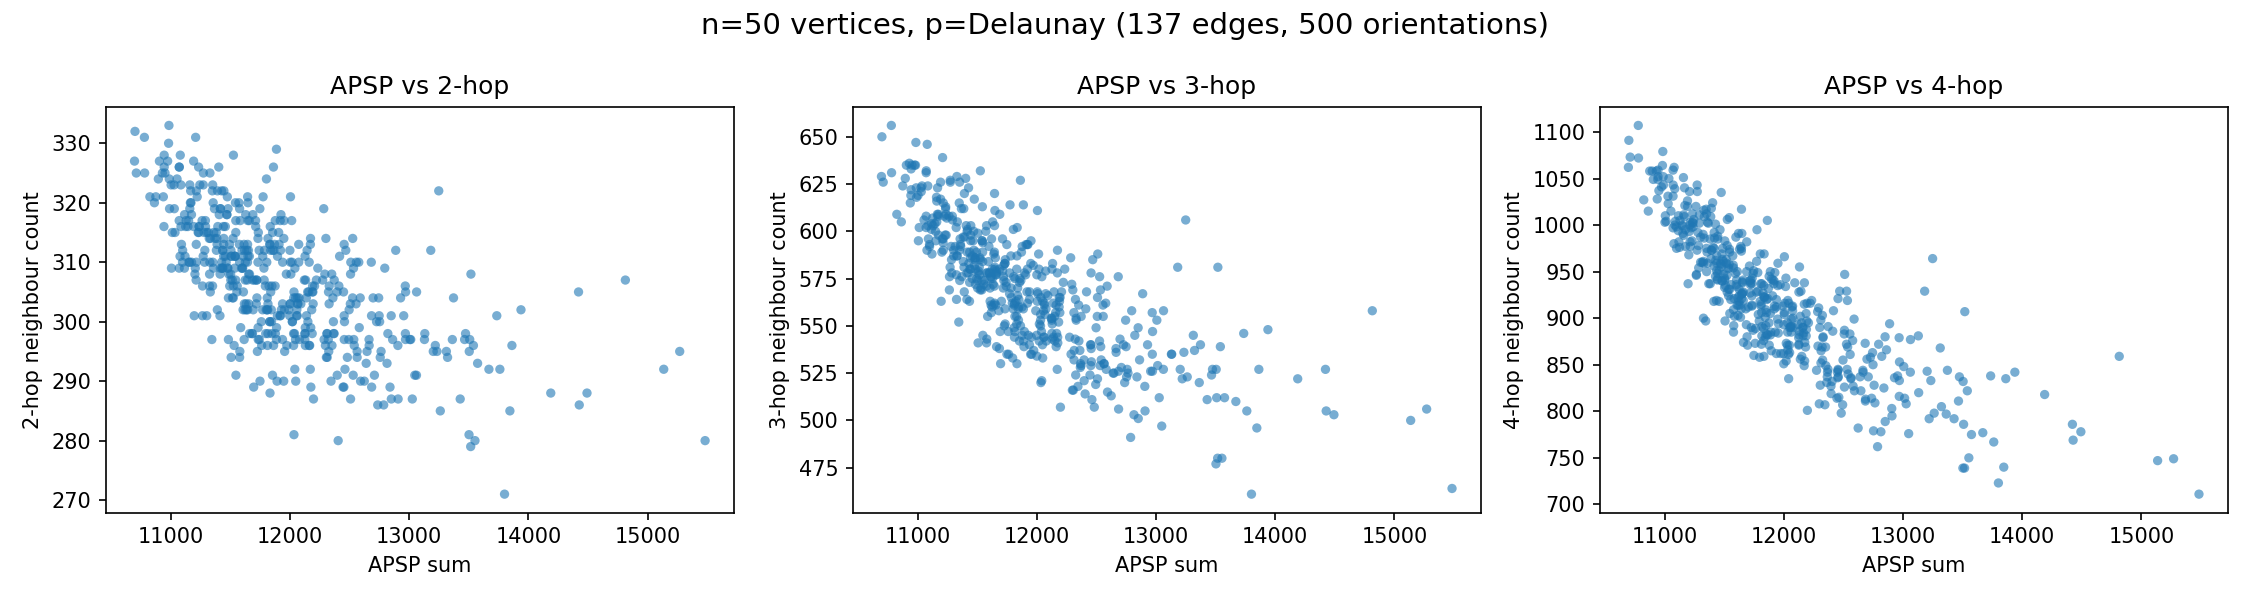
\includegraphics[width=0.85\textwidth]{result_v50_Delaunay.png}
    \caption{$n=50$에서의 n-hop 이웃 수 합과 APSP 총합의 상관관계}
    \label{fig:n50}
\end{figure}

\begin{figure}[t]
    \centering
    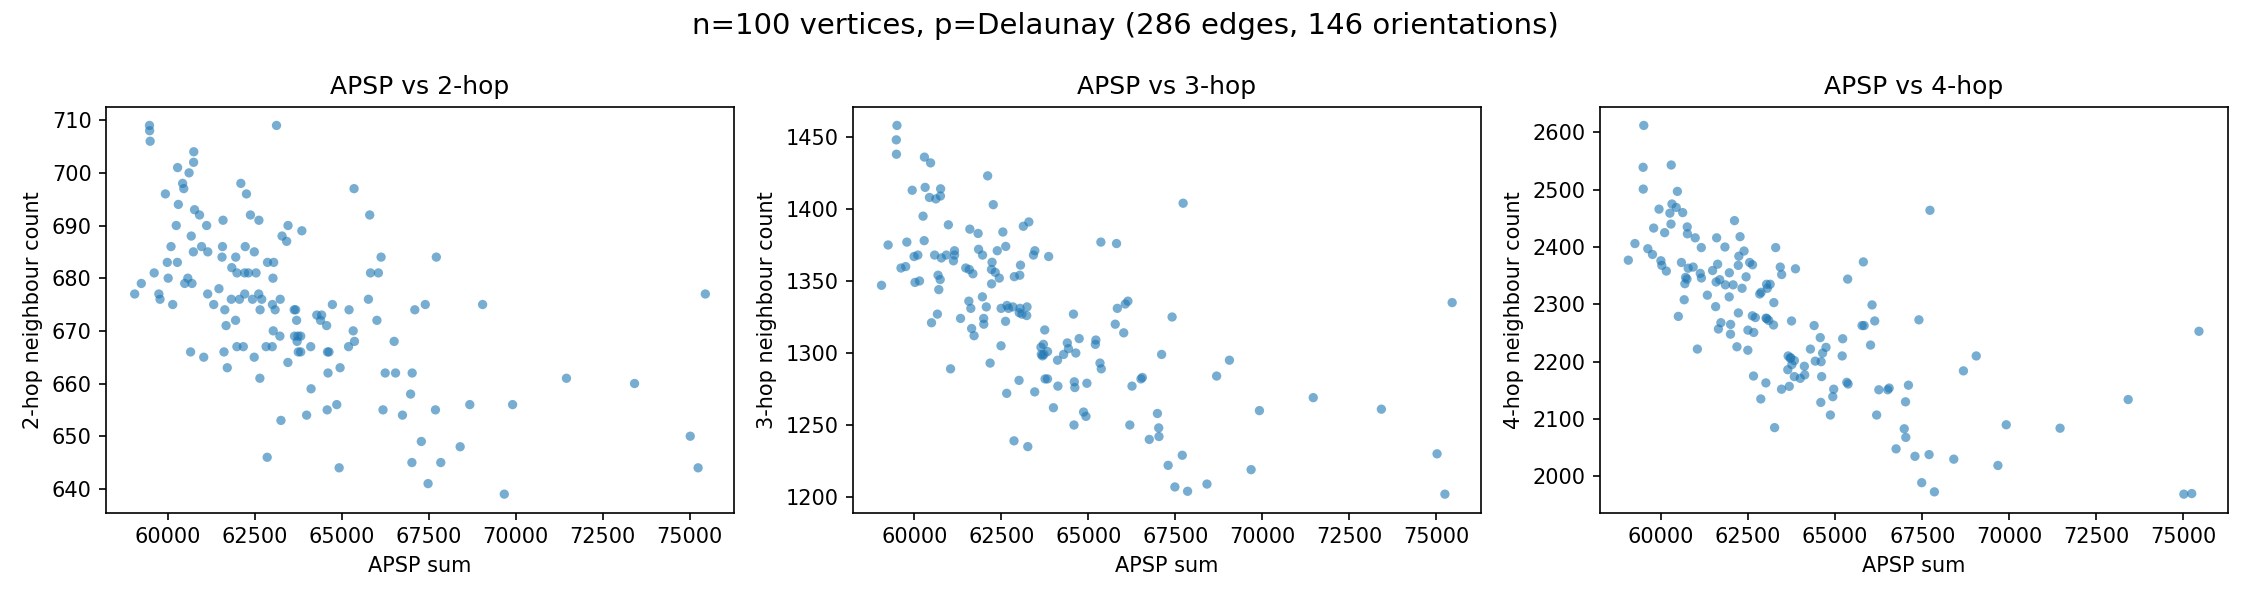
\includegraphics[width=0.85\textwidth]{result_v100_Delaunay.png}
    \caption{$n=100$에서의 n-hop 이웃 수 합과 APSP 총합의 상관관계}
    \label{fig:n100}
\end{figure}

Figure~\ref{fig:n10}, \ref{fig:n50}, \ref{fig:n100}에서 보듯,
노드 규모와 관계없이 $n$-hop 이웃 수가 증가함에 따라
APSP 총합이 감소하는 강한 음의 상관관계가 관찰됩니다.
이를 기반으로 $H_{dist}$를 다음과 같이 설계하였습니다:
\begin{equation}
H_{dist} = - \sum_{\forall e_{ik}, e_{kj}}(I_{i\rightarrow k} I_{k\rightarrow j}) - \sum_{\forall e_{ij}, e_{jk}, e_{kl}}(I_{i\rightarrow j} I_{j\rightarrow k} I_{k\rightarrow l})
\end{equation}

\section{구현 및 실험}

\subsection{차수 감소 및 구현}
$H_{dist}$의 고차 항을 2차 형식으로 변환하기 위해 D-Wave Ocean SDK의 \texttt{dimod.\allowbreak make\_quadratic} 기능을 활용하였습니다. 이는 Rosenberg(1975) 등이 제안한 페널티 기반 차수 감소(Degree Reduction) 기법을 기반으로 보조 변수를 도입하여 모델의 수치적 엄밀함을 확보합니다.\cite{glover2018tutorial}

\subsection{성능 평가 결과}
제안된 MR2S 모델을 Raw SA 및 전수 조사(Bruteforce) 방식과 비교한 결과입니다.

\paragraph{노드 규모별 벤치마크 결과}
\begin{table}[ht]
\centering
\subcaption*{[Case 1] 노드 5개 (간선 8개)}
\begin{tabular}{|l|c|c|c|c|c|}
    \hline
    그래프 유형 & 최소 APSP 합 & 평균 APSP 합 & 평균 $\sum(In-Out)^2$ & 시간(ms) \\ \hline
    \textbf{MR2S} & 34 & 34.00 & 4.00 & 224.26 \\ \hline
    \textbf{Raw} & 34 & 34.00 & 4.00 & 205.41 \\ \hline
    \textbf{Bruteforce} & 34 & 34.00 & 4.00 & 103.12 \\ \hline
\end{tabular}

\vspace{0.3cm}
\subcaption*{[Case 2] 노드 10개 (간선 19개)}
\begin{tabular}{|l|c|c|c|c|c|}
    \hline
    그래프 유형 & 최소 APSP 합 & 평균 APSP 합 & 평균 $\sum(In-Out)^2$ & 시간(ms) \\ \hline
    \textbf{MR2S} & 206 & 207.50 & 6.00 & 389.75 \\ \hline
    \textbf{Raw} & 206 & 209.00 & 6.40 & 560.96 \\ \hline
    \textbf{Bruteforce} & N/A & N/A & N/A & 11019.55 \\ \hline
\end{tabular}

\vspace{0.3cm}
\subcaption*{[Case 3] 노드 20개 (간선 45개)}
\begin{tabular}{|l|c|c|c|c|c|}
    \hline
    그래프 유형 & 최소 APSP 합 & 평균 APSP 합 & 평균 $\sum(In-Out)^2$ & 시간(ms) \\ \hline
    \textbf{MR2S} & 1094 & 1094.00 & 8.00 & 421.91 \\ \hline
    \textbf{Raw} & 1083 & 1100.20 & 9.20 & 1324.08 \\ \hline
    \textbf{Bruteforce} & N/A & N/A & N/A & 15152.42 \\ \hline
\end{tabular}
\end{table}

\subsubsection{결과 분석 및 향후 계획}
실험 결과, 본 연구에서 제안한 $n$-hop 및 APSP 근사 방식은 기존의 시뮬레이션 어닐링(Raw SA)보다 실제 보행 효율성 및 연산 속도 측면에서 더욱 우수한 성능을 보여주었습니다. 특히 대규모 그래프로 갈수록 안정적인 최적해 도출 능력이 확인되었습니다.

마지막으로, 본 연구팀은 오제키 교수님(Prof. Ozeki)으로부터 실제 양자 어닐링(QA) 하드웨어에 대한 접근 권한을 지원받기로 하였습니다. 이에 따라 실제 QA 시스템 상에서 본 QUBO 모델의 하드웨어 가속 성능을 측정하고 검증하는 과정을 통해 최종 성과를 도출할 예정입니다.

\section{결론}
본 연구는 보행자 안전 문제를 양자 어닐링으로 정형화하여 동선 최적화의 새로운 가능성을 제시하였습니다. 향후 실제 도시 데이터를 기반으로 한 연구를 지속하며, QA 하드웨어 검증을 통해 실시간 안전 시스템으로의 발전을 도모할 것입니다.

% 참고문헌 스타일 설정 (IEEEtran, plain, unsrt 중 선택)
\bibliographystyle{unsrt} 
% .bib 파일 이름 입력 (확장자 제외)
\bibliography{references}

\end{document}